\begin{itemize}
	\item Мы решаем однородное уравнение на величину $C_i(t) = \deriv{N}{t}$, которое описывает эволюцию частиц, захватившихся за единицу времени в момент $t=0$.
\end{itemize}

\begin{figure}
	\centering
	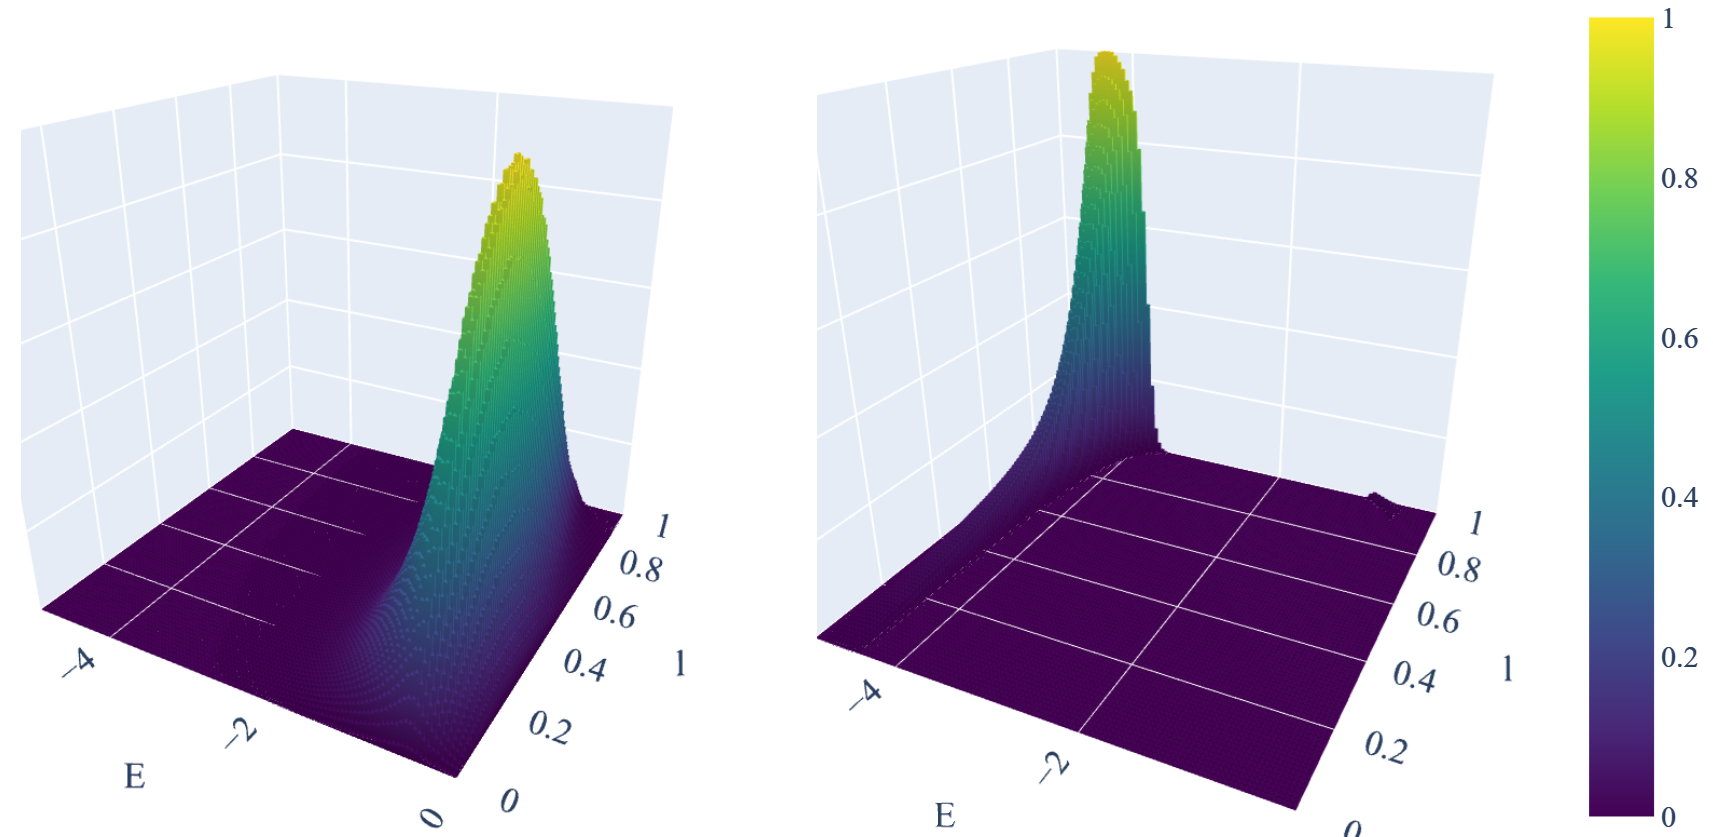
\includegraphics[width=0.7\textwidth]
	{images/Capt100_100.png}
	\caption{Распределение захваченных частиц для $m_{\chi} = 100\, \text{GeV}$, $\delta = 100\, \text{keV}$.}
\end{figure}